\documentclass[final]{beamer}
% beamer 3.10: do NOT use option hyperref={pdfpagelabels=false} !
% \documentclass[final,hyperref={pdfpagelabels=false}]{beamer} 
% beamer 3.07: get rid of beamer warnings

\mode<presentation> {  
%% check http://www-i6.informatik.rwth-aachen.de/~dreuw/latexbeamerposter.php for examples
  \usetheme{Durham} %% This points to the theme cooked up by the final year tutor
}


\usepackage[english]{babel} 
\usepackage[latin1]{inputenc}
\usepackage{amsmath,amsthm, amssymb, latexsym}
\usepackage{subfigure}
\usepackage{savetrees}
  \usefonttheme[onlymath]{serif}
  \boldmath
  \usepackage[orientation=portrait,size=a3,scale=1.4,debug]{beamerposter}                       

  % e.g. for DIN-A0 poster
  % \usepackage[orientation=portrait,size=a1,scale=1.4,grid,debug]{beamerposter}
  % e.g. for DIN-A1 poster, with optional grid and debug output
  % \usepackage[size=custom,width=200,height=120,scale=2,debug]{beamerposter} % e.g. for custom size poster
  % \usepackage[orientation=portrait,size=a0,scale=1.0,printer=rwth-glossy-uv.df]{beamerposter}
  % e.g. for DIN-A0 poster with rwth-glossy-uv printer check ...
  %

  \title[Final Year Project Poster]{Cloud-based RAW Image Editing}
  \author[R Collins]{Ryan Collins}
  \institute[Durham]{Department of Computer Science, Durham University}
  \date{\today}

  \begin{document}
  \begin{frame}{} 

  \vfill
    \begin{columns}[t]
      \begin{column}{.48\linewidth}
        \begin{block}{Introduction}

          This poster describes the design and implementation of
          a Cloud-based system for processing and editing RAW images.
          Previous RAW image editing software is designed for native
          use, and most of the current software available is proprietary.
          This paper shows the design and implementation of a system
          that's not proprietary, and allows for editing of RAW images
          through our Cloud-based RAW image editing service.

        \end{block}

        \begin{block}{RAW Images Explained}
          RAW isn't a file format in itself, but rather an umbrella term for a set of many different formats that store the
          raw camera sensor data. There are a set of different proprietary file formats, that all store similar information,
          but in different ways.
          
          When an image is captured, the camera sensor uses charge buildup to represent the amount of light that is incident on the sensor
          (using a phenomenon known as the photoelectric effect). Colour data itself isn't stored at all in the RAW image. Colour is achieved
          by putting a filter over the sensor, such that each individual part of the sensor captures only red, green or blue light, which then
          allows one to build up a full colour image. The process of creating a full colour image from the camera sensor is called demosaicing.
          
          
          There are several different steps to decoding RAW images, in addition to demosaicing which was explained above. These are:
          \begin{itemize}

          \item \textbf{White Balance}
          
          
          \item \textbf{Gamma Correction}
          Cameras typically represent colour changes linearly, with a gamma of 1.0.
          However, this isn't necessarily pleasing to the eye, so this can be changed to change how tones are reflected. This can be used to simulate
          the tonal output of film cameras, for example.
          
          \item \textbf{Sharpening/Noise Reduction}
          Sometimes, noise can creep into the image, particularly if the image itself is shot with large ISO levels (ISO is a sensitivity setting that can be
          set when taking a photo, to allow the camera sensor to be more sensitive to light). This can be corrected
          during the editing process.
          
          Also, sometimes edges might need to be enhanced to bring out the detail in the image. This can again be used for stylistic purposes, but this is ultimately the
          decision of the image editor.
          \end{itemize}
        \end{block}
       
        \begin{block}{Test of Exposure Adjustment}
          \begin{figure}\label{exposuretest}
            \centering
            \subfigure
            {
                \includegraphics[width=75px]{brightnesspoint0001}
            }
            \subfigure
            {
                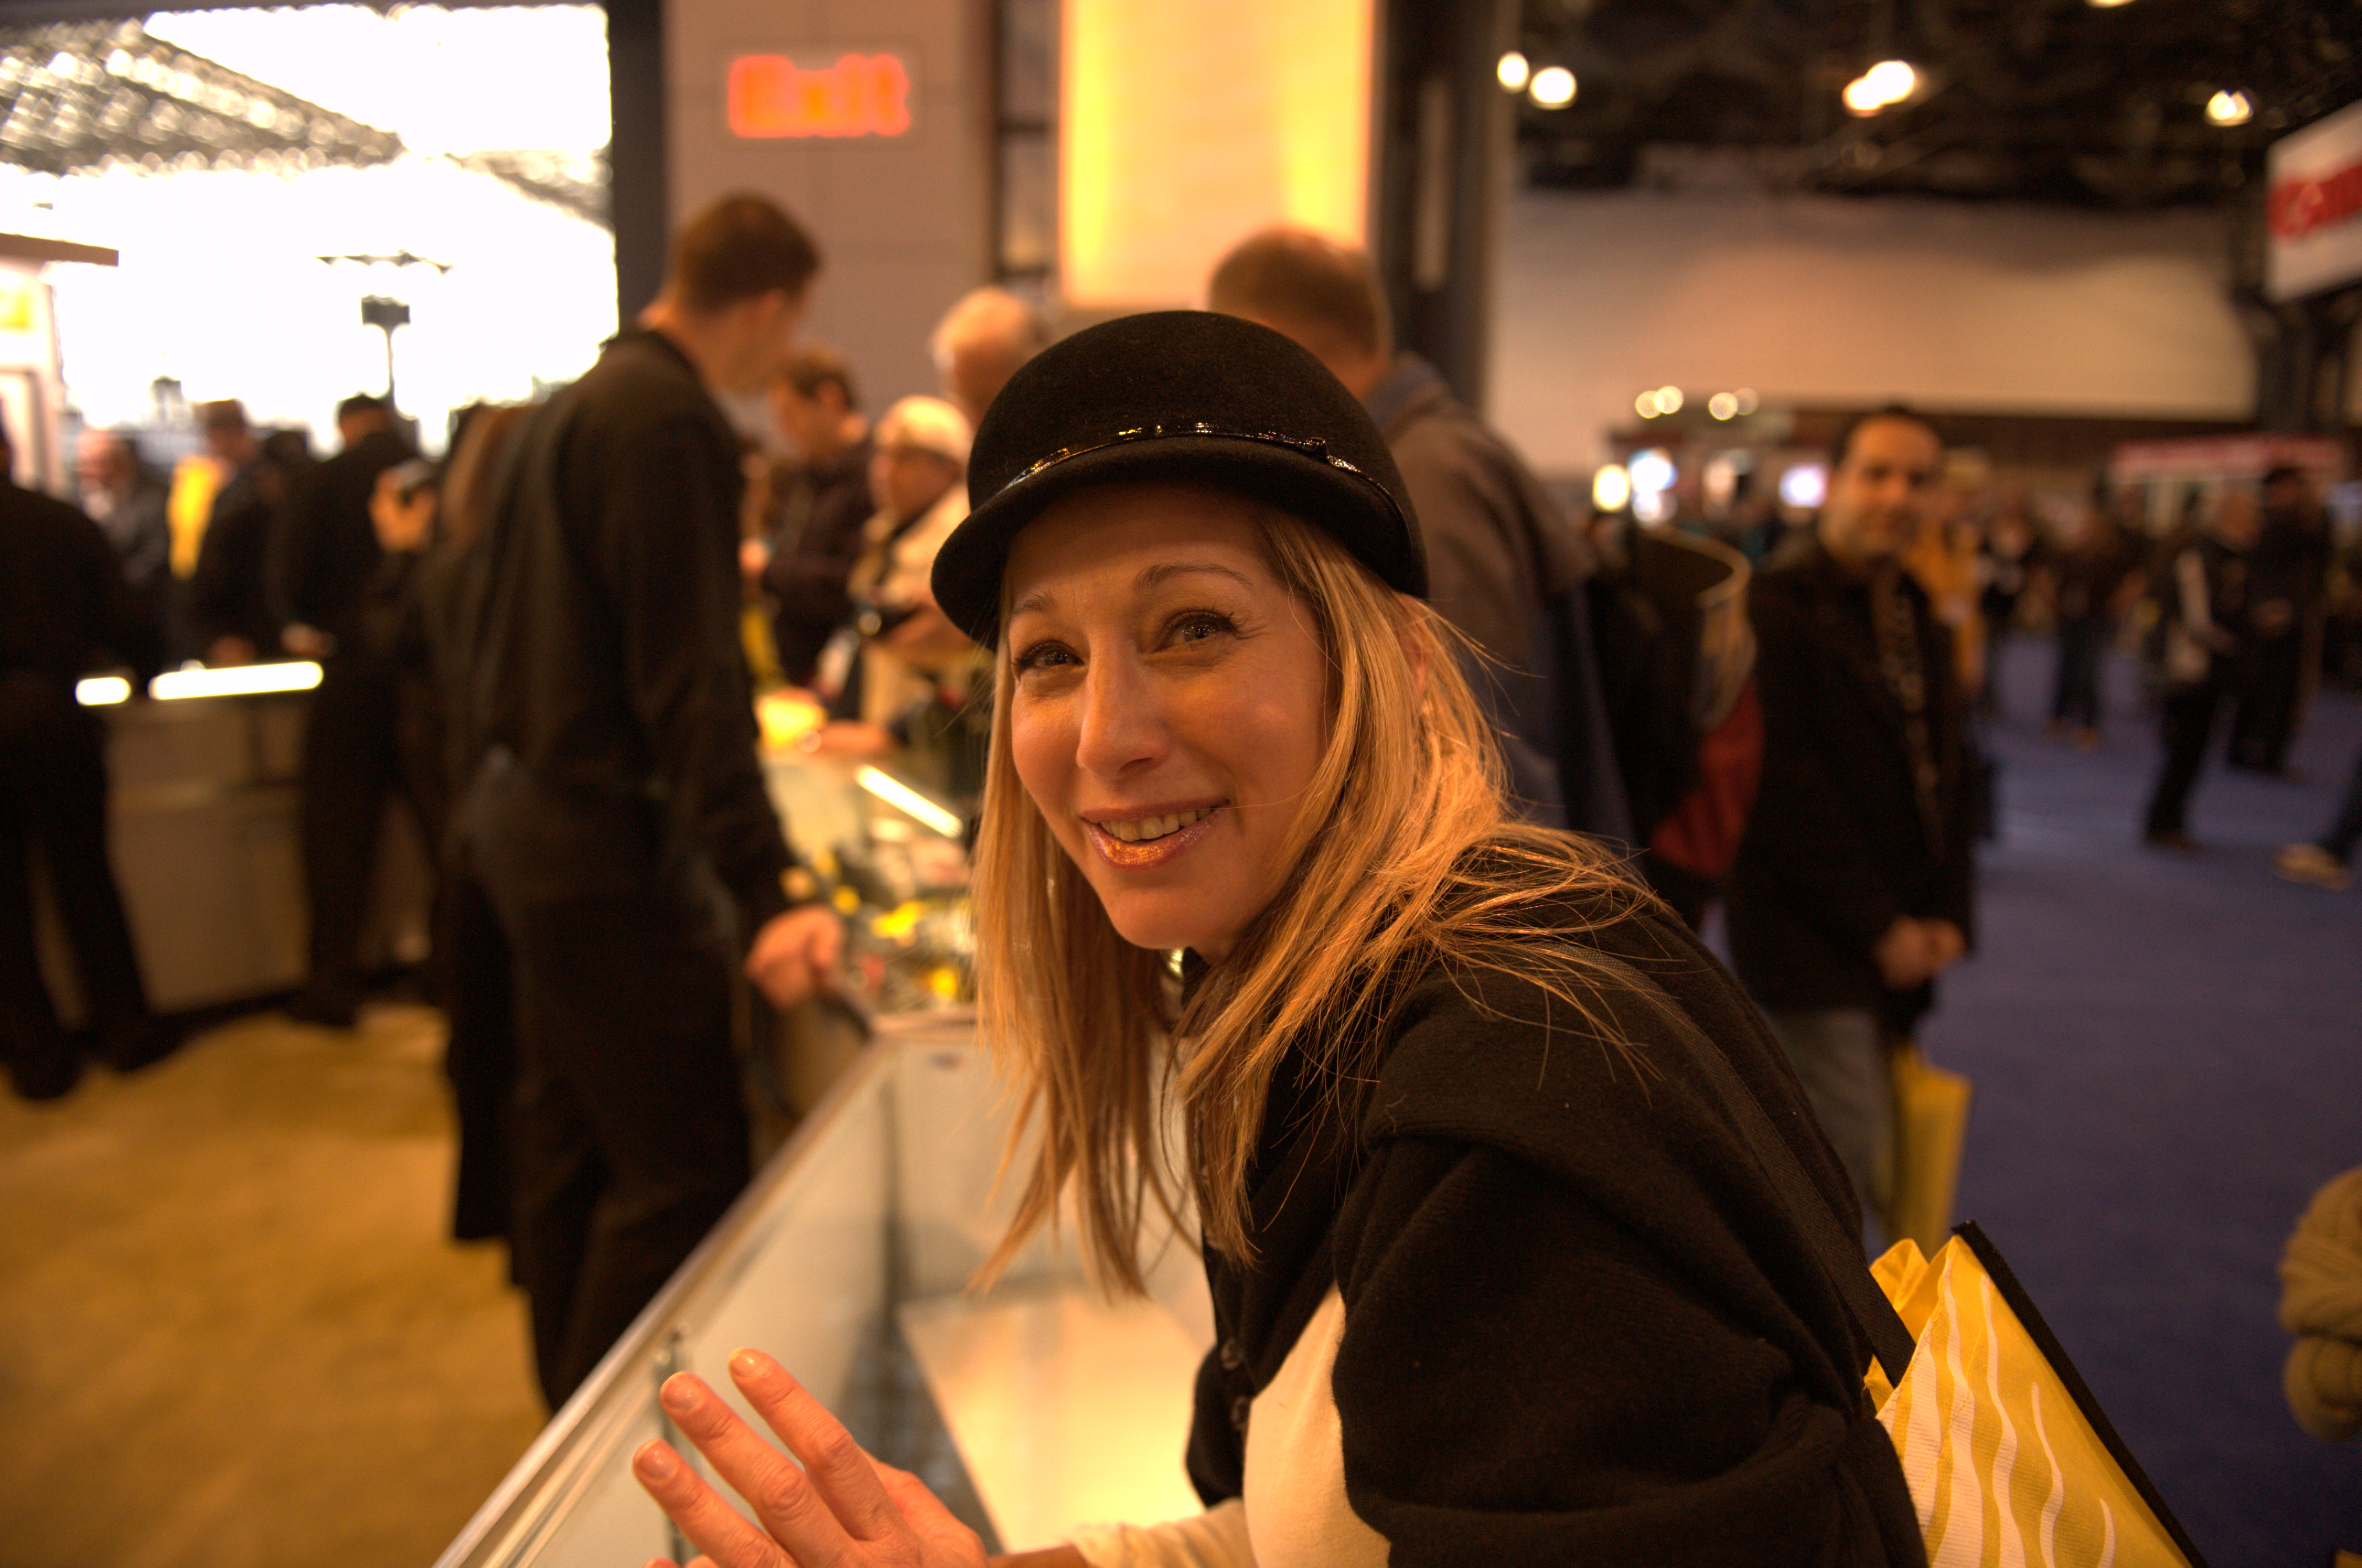
\includegraphics[width=75px]{brightnessnormal}
            }
            \subfigure
            {
                \includegraphics[width=75px]{brightness5000}
            }
            \caption{
                Test of Exposure Adjustment 
                (a) Exposure Level Small: 0.0001
                (b) Exposure normal: 1.0
                (c) Exposure level high: 5000
            }
         \end{figure}

        \end{block}

        \begin{block}{Test of Colour Adjustment}
          \begin{figure}\label{colourbalancetest}
            \centering
            \subfigure
            {
                \includegraphics[width=75px]{colourtest_no_adjustment}
            }
            \subfigure
            {
                \includegraphics[width=75px]{colourtest_redonly}
            }
            \subfigure
            {
                \includegraphics[width=75px]{colourtest_greenonly}
            }
            \subfigure
            {
                \includegraphics[width=75px]{blueonly}
            }
            \caption{
                Test of Colour Balance 
                (a) No Adjustment
                (b) Red only (green and blue zero)
                (c) Green only (red and blue zero)
                (d) Blue only (red and green zero)
            }
         \end{figure}
         To test the functionality of colour adjustment, we can compare the output of only one channel.
         If the outcome is only the specified channel, then the colour balance component of the system works.
        \end{block}

        \begin{block}{Test of Gamma Correction}
          \begin{figure}\label{gammatest}
            \centering
            \subfigure
            {
                \includegraphics[width=100px]{gammacorrectionlow}
            }
            \subfigure
            {
                \includegraphics[width=100px]{gammacorrection_normal}
            }
            \subfigure
            {
                \includegraphics[width=100px]{gammacorrectionhigh}
            }
            \caption{
                Test of Gamma Correction output. 
                (a) $\gamma = 0.3$
                (b) $\gamma = 1.0$
                (c) $\gamma = 1.7$
            }
         \end{figure}
        \end{block}


      \end{column}


      \begin{column}{.48\linewidth}


        \begin{block}{Overall System Workflow}
          \includegraphics[width=\columnwidth]{DesignSystemandGA}
        \end{block}
        \begin{block}{System Workflow Explained}

          The system shall receive a set of instructions, encoded using the JavaScript
          Object Notation (JSON). These instructions outline what RAW image to use, along with
          the settings to use for rendering.

          Due to the proprietary nature of RAW files, rolling our own RAW processing engine is not
          advisable, as each camera manufacturer has a different file format, and there isn't really
          an agreed on standard. While one could use Adobe's standard DNG, converters to DNG only exist
          for Windows and Mac, not Linux (which various Cloud systems might rely on). Therefore, an
          executable called Dcraw (which is a self-contained C file containing no dependencies) is used
          to preprocess the RAW image into an uncompressed TIFF image, which is readable by many programming
          languages as an image file. While Dcraw isn't directly portable, as the executable doesn't require
          any external dependencies, it massively simplifies the build process, and providing a C compiler exists
          for some platform, building of this executable can be done automatically (or the external executable can be
          alternatively obtained from a package manager). 

        \end{block}

        

      \end{column}
    \end{columns}

  % \vfill
  %   \begin{block}{\large This shows different font sizes you can use}
  %     \centering
  %     {\tiny tiny}\par
  %     {\scriptsize scriptsize}\par
  %     {\footnotesize footnotesize}\par
  %     {\normalsize normalsize}\par
  %     {\large large}\par
  %     {\Large Large}\par
  %     {\LARGE LARGE}\par
  %     {\veryHuge VeryHuge}\par
  %     {\VeryHuge VeryHuge}\par
  %     {\VERYHuge VERYHuge}\par
  %   \end{block}
  %   \vfill

  \end{frame}
\end{document}


